\section{g-h Filter}

\subsection{Intuition}
\begin{frame}
   \frametitle{Intuition}

		\begin{itemize}
			\item Any measurement is inaccurate.
			\item This is the motivation behind a huge body of work in filtering.
			\item Suppose that we have one billion of sensor readings for today's temperature, How could we choose to announce a fixed value?
			\item Yes. The answer is averaging. In estimation theory, it recalls as the expected value. 
			\item More formally, the first moment of a random variable (average) is the best estimator for now. 
		\end{itemize}
		
		\begin{figure}
		\centering
			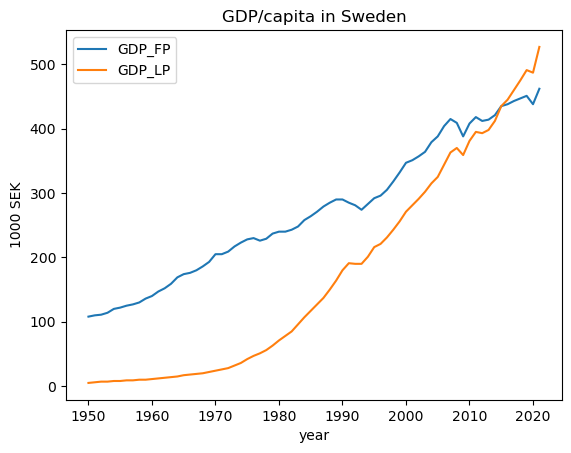
\includegraphics[width=0.40\textwidth]{Figures/g-h_filter/GDP.png}
		\label{gdp}
		\caption{fig: Sweden gross domestic product, we use this dataset for making our g-h filter}
	\end{figure}
	This is where it all started: \cite{labbe2014kalman}	
\end{frame}
%-----------------------------------------------------¨

\subsection{Data preprocessing}
\begin{frame}[fragile]
   \frametitle{Data preprocessing}
	
\begin{minted}{python}
y = df['GDP_LP'][-22:-1].to_list() #read variable in Pandas datafraeme format
x = range(1, len(y)+1) 
tick = df.index[-22:-1]
coefficients = np.polyfit(x, y, 1)  # Fit a first-order polynomial (line)
fit_function = np.poly1d(coefficients) #calculate prediction after fitting a red line

fig, ax = plt.subplots(figsize=(12,4)) #read about matplotlib.pyplot
ax.scatter(x, y, label='GDPs')
yerr = [element * 0.03 for element in y]
ax.errorbar(x, y, fmt='o', xerr=0, yerr=yerr, capthick=2, capsize=10)
ax.plot(x, fit_function(x), color='red', label='Least Squares Fit')
ax.set_xlabel('year')
ax.set_ylabel('1000 SEK')
ax.set_xticks(x, tick)
plt.title('Sweden GDP/captia in the one-fifth of 20 century')
plt.legend();
fig.tight_layout()
\end{minted}

\end{frame}

\subsection{Data visualization}
\begin{frame}
   \frametitle{Data visualization}


   		\begin{figure}
		\centering
			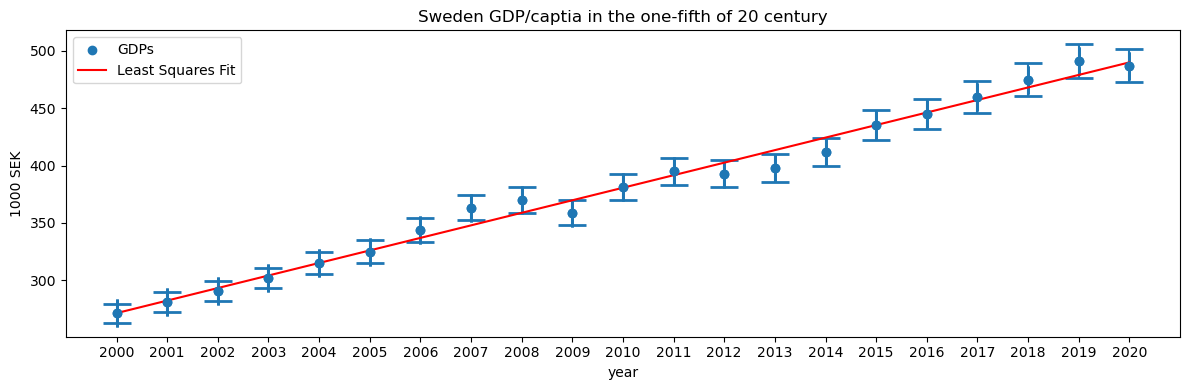
\includegraphics[width=1\textwidth]{Figures/g-h_filter/data_vis.png}
		\label{data_vis}
	\end{figure}

 \end{frame}
 
\subsection{g-h function}

\begin{minted}{python}
def g_h_filter(data, X0, dx, g, h, dt=1., do_print = True):
    x_est = X0
    estimates, predictions = [x_est], []
    for z in data:
        # prediction step
        x_pred = x_est + (dx*dt)
        dx = dx

        # update step
        residual = z - x_pred
        dx = dx + h * (residual) / dt
        x_est = x_pred + g * residual
        predictions.append(x_pred)
        estimates.append(x_est)
        if do_print:
            print('previous estimate: {:.2f}, prediction: {:.2f}, estimate {:.2f}'.format(estimates[-2], x_pred, z))
    return np.array(estimates), np.array(predictions)

estimates, preds = g_h_filter(data=y, X0=270., dx=10., g=6./10, h=2./3, dt=1.)
\end{minted}

\end{frame}

\begin{frame}
   \frametitle{g-h filter performance}

   The estimates are not a straight line, but they are straighter than the measurements and somewhat close to the trend line we created. Also, it seems to get better over time.

   		\begin{figure}
		\centering
			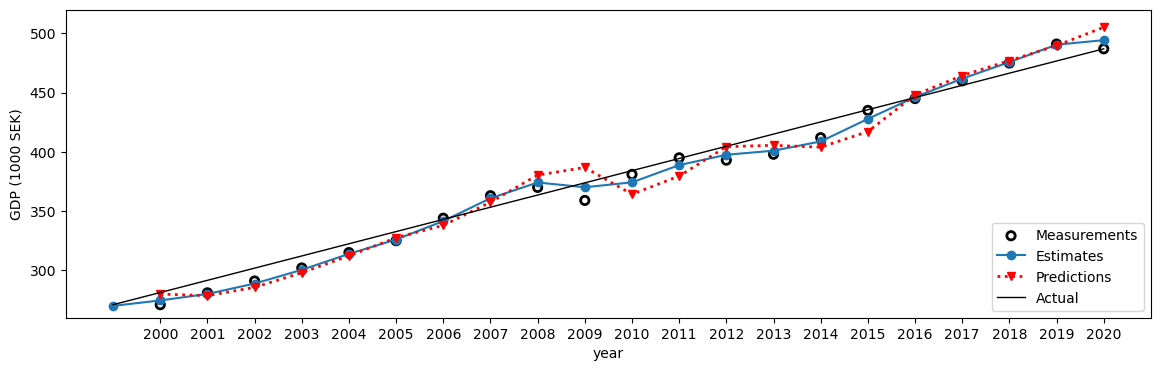
\includegraphics[width=1\textwidth]{Figures/g-h_filter/g-h-filter-res.png}
		\label{gh_res}
	\end{figure}

 \end{frame}

